\documentclass[tikz]{standalone}

\input{../tikz.tex.preamble}
\input{../typography.tex.preamble}

\begin{document}
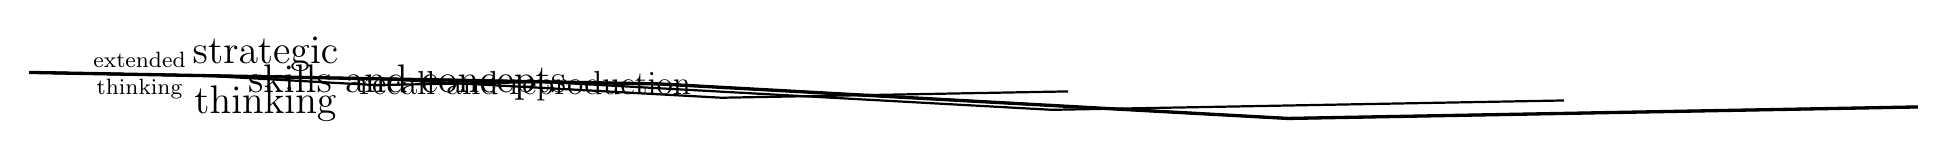
\begin{tikzpicture}[x=2cm, y=2cm]
  \draw[thick] (0,0) --++ ({-pi/3}:1.1) --++({-pi}:1.1) --++({pi/3}:1.1);
  \node at ({-pi/2}:0.7) {\parbox{2cm}{\footnotesize \centering extended\\ thinking}};
  \draw[thick] (0,0) --++ ({-pi/3}:2.2) --++({-pi}:2.2) --++({pi/3}:2.2);
  \node at ({-pi/2}:1.5) {\parbox{2cm}{\centering \Large strategic\\ thinking}};
  \draw[thick] (0,0) --++ ({-pi/3}:3.25) --++({-pi}:3.25) --++({pi/3}:3.25);
  \node at ({-pi/2}:2.4) {\Large skills and concepts};
  \draw[thick] (0,0) --++ ({-pi/3}:4) --++({-pi}:4) --++({pi/3}:4);
  \node at ({-pi/2}:3.15) {\large recall and reproduction};
  \draw[very thick] (0,0) --++ ({-pi/3}:4) --++({-pi}:4) --++({pi/3}:4);
\end{tikzpicture}
\end{document}
